\section{Strukturorientierte Testverfahren}

\begin{tcolorbox}[title=Strukturorientierte Testverfahren]
    Bei \textbf{strukturorientierten Testverfahren}, auch \textbf{White-Box-Tests} genannt, wird zur \textbf{Konstruktion der Testfälle} als auch zur \textbf{Bestimmung der Vollständigkeit} der Tests der Quellcode herangezogen.\\
    Dadurch soll sichergestellt werden, dass jede existierende Codezeile in Tests ausgeführt worden ist.
\end{tcolorbox}



\begin{figure}
    \centering
    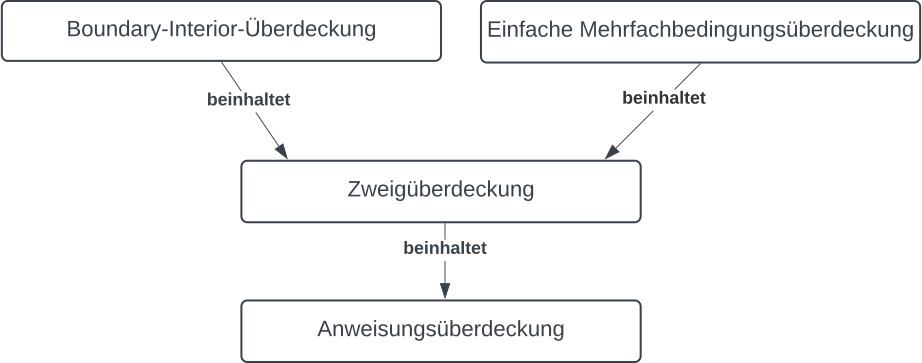
\includegraphics[scale=0.4]{part four/Testende Verfahren/img/coverage-criteria-hierarchy}
    \caption{Hierarchie der verschiedenen Überdeckungskriterien. (Quelle: in Anlehnung an \cite[Abb. 5.2, 53]{Wed09c})}
    \label{fig:coverage-criteria-hierarchy-cc}
\end{figure}